SeatGen uses a save button to save the currently edited state and changes in the map. This has some advantages and disadvantages compared to saving every time an action occurs. Some advantages are:

\textbf{Advantages:}
\begin{compactitem}
    \item The user can undo changes without saving them
    \item The user can save the changes when they are done, and try them without saving, while not overwriting the last state.
    \item There is less load on the server, because multiple changes are saved at once
    \item Unnecessary load is avoided when doing a lot of small changes in a short time
    \item Only the important changes are saved, and not every step in between
\end{compactitem}

\textbf{Disadvantages:}
\begin{compactitem}
\item If the user forgets to save, all changes are lost
\item There is an extra step the user has to execute
\end{compactitem}

To mitigate these disadvantages, SeatGen uses some techniques, like when the user tries to leave the page by reloading or closing the tab, the browser will ask the user if they are sure that they want to leave the page, because there are unsaved changes. This is done by using the \texttt{beforeunload} event, which is triggered when the user tries to leave the page. This event is used to show a confirmation dialog to the user, which asks if they are sure they want to leave the page (Figure \ref{fig:save-button}).

\begin{figure}
    \centering
    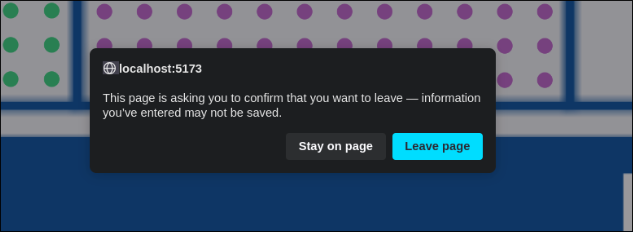
\includegraphics[scale=0.5]{pics/save-button.png}
    \caption{Leave Confirmation Dialog}
    \label{fig:save-button}
\end{figure}

To ensure that the user does not forget to save, the save button is always visible, and always when the user has made changes, the save button is highlighted as seen in Listing \ref{fig:save-button-states}. This is done by the controller that manages the undo and redo functionality that is explained in section \ref{sec:undo-redo}. The code in listing \ref{lst:check-unsaved-changes} checks if there have been any actions by the user that are not at the currently saved index, or if there are any standing areas that have to be saved or deleted. The standing areas have been managed differently for technical reasons.

\begin{figure}
    \centering
    
\includegraphics[scale=0.4]{pics/save-button-states.png}
    \caption{Save Button States}
    \label{fig:save-button-states}
\end{figure}

\begin{lstlisting}[language=TypeScript, caption=Check for Unsaved Changes, label=lst:check-unsaved-changes]
function checkForUnsavedChanges() {
    setHasUnsavedChanges(
        historyIndex !== savedIndex ||
        standingAreasToSave.length != 0 ||
        standingAreasToDelete.length != 0
    )
}
\end{lstlisting}

When saving the changes, first a checksum that is the hash of all seats and their properties is calculated and compared to the checksum of the initial loading of the map. If the checksums are the same, no seats will be saved, because they didn't change. If the checksum is different, a snapshot of the current seats is sent to the backend for saving. For the standing areas there are two variables. \texttt{standingAreasToSave} and \texttt{standinAreasToDelete}. These are set relative to the last saved state. When saving, the \texttt{toSave} items are saved in the backend, and the \texttt{toDelete} items are deleted. After the save is successful both variables are empty. When creating a new standing area or deleting an existing one, the variables get filled with the respective standing area. A big advantage over saving every time an action occurs is that when creating and then deleting an area without saving in between, there are no unsaved changes, and no traffic has to be sent, because the final state is the same as before.